\section{Sprint Planning}
After assembling all the tools in Sprint0, we decided to start with the implementation of core modules.
As our understanding of task improved, we were able to come up with user stories from the perspective of user, customer, developer and student.
All user-stories were given to the customer so they can be prioritized. 
All but user-stories concerning our student obligations, like writing project plan, minutes, meetings with supervisor and attending lectures.
We decided to have school tasks as a user stories so we can better keep our time tracking. 
Those were mandatory and already added as user-stories of sprint1.
On Monday 02.09.2013. we had the meeting with a customer where we estimated time we need for every user story.
The result of that meeting was the list of the rest of the user-stories for sprin1.
We agreed date for presentation and showing the running demo - Thursday 12.09.2013.

\subsection{Sprint1 User-stories}

\LTXtable{\textwidth}{sprint1/stories.tex}

\section{Sprint Goal}
We decoupled user-stories into tasks and we were ready to start with the implementation of client-server core module.
This core module will offer only communication and the most basic system operations. 
Our goal is to deliver working demo over core module including registering service, listening for the clients and send simple signals to the client from the server.
And scaning for the services, connecting, recieving signals and play commands on the client. 

\section{Architecture}

For the core communication and organisaton of our product we selected Client-Server Arhitecture.
Choosing this arhitecture was very intuitive to do as our project should consist of two applications and overall tasks should be partitioned. 
Client application should be able to light up different sequences of lights depending on server command signals.
And server application should be responsable for awaiting incoming clients connections, mapping clients to the grid and providing command play signals to the clients by brodcast.
Communication should be established over computer network using same router for both applications, the user and the server, and wihout need for third party server or internet connection. 


Our first research of technologies that could help as at achiving client-server communication, without writing everything from strach, was Bonjur software. 
It is the Apple's implementation of Zero configuration network (Zeroconf). 
Zero-configuration network (Zeroconf)  is a methodology and a set of special technologies that automatically create a usable computer network based on the Internet Protocol Suite (TCP/IP) when computers or network peripherals are interconnected. 
It does not require manual operator intervention or special configuration servers.
It is assembled of technologies that includes service discovery, addressing assigment, and hostname resolution.
Aldo good and very usefull tool it is not suported on Android, and since Android is our platform of choise we had to research further. 
We learned that we want zeroconf library with similar set of services as Bonjur writen in Java.


Further research brought us to JmDNS. Java imaplementation of multi-cast DNS that can be used for service registration and discovery in Local Area Network. 
It works on most JDK1.6 compatibile Virtual Machines, it comes as a library and it is easy to intigrate with Android. 
JmDNS fullfill all of our expetations, but while learning about it over internet, we found that Android itself have built in Nestwork Service Discovery(NSD) that do the same thing.


Android Network Service Discovery(NSD) is supported from API version 16. 
It allows users to identify other devices on the local network, register services, broadcast connection information, scan for registered services and connect.
Even with minimum API limitation it is a part of Android platform, no third part libreries are needed, it will evolve with Android and therefore always be working.
Min API version was not of concern to the customer as he replied on mail regarding this question, so we made a decision of using Android Network Discovery(NSD) for client-server descovery and communication.

NSD send look like this:

Device Identifier: HelloWorldServer
Service Name: \_helloWorld.\_tcp.
Port: 27812
Network Address: 192.168.1.31

explain sockets

\begin{figure}[!t]
	\centering
		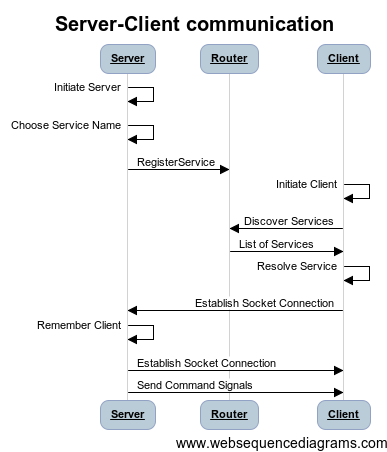
\includegraphics[width=10cm]{sprint1/Server-Client communication.png}
	\caption{Sprint1 Arhitecture}
	\label{fig:sprint1_arhitecture}
\end{figure}



\begin{figure}[!t]
	\centering
		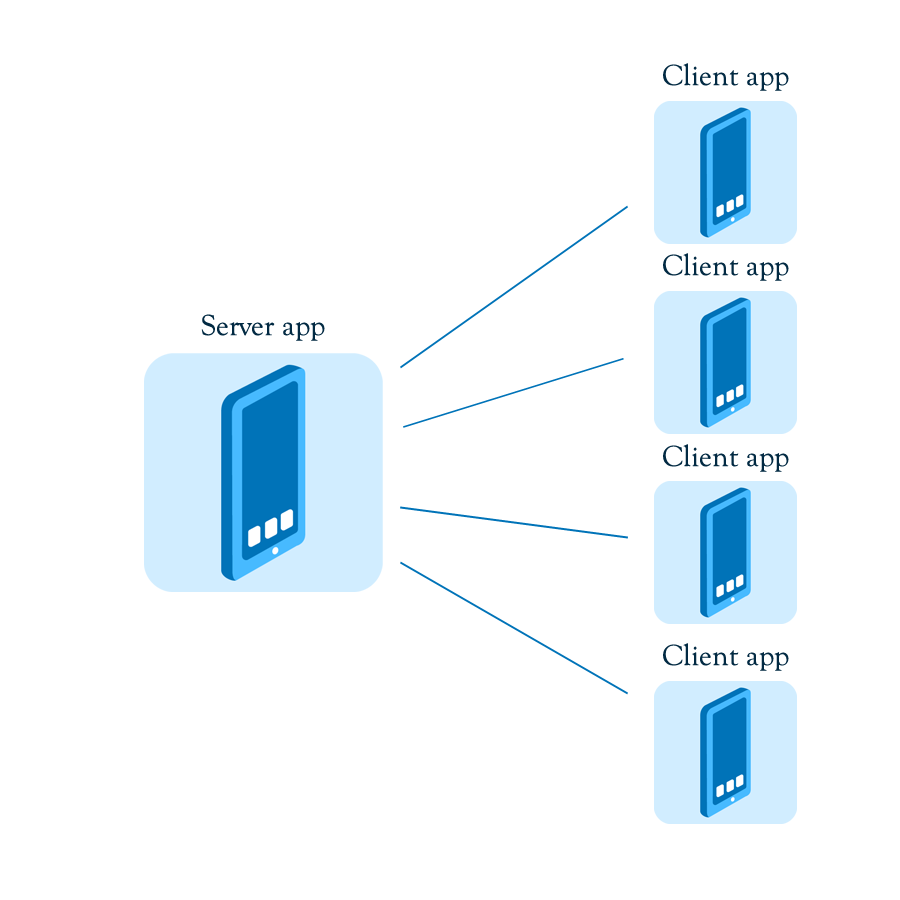
\includegraphics[width=16cm]{sprint1/arhitecture.png}
	\caption{Sprint1 Arhitecture}
	\label{fig:sprint1_arhitecture}
\end{figure}

\section{Implementation}

NSD
\section{Testing}

\section{Occurring risks}

That Android will not get NSD able for low APIs. 
Then we have to use third part libreries.

\section{Retrospective}
\subsection{Pros}
\subsection{Cons}
\section{Evaluation}
